Denne seksjonen tar for seg Porters fem krefter og PESTEL- analyse, som gir innsikt i byggisolasjonsbransjen og bedriftens makroomgivelser. Analysene kartlegger eventuelle trusler og muligheter bedriften står overfor i tiden fremover.

\section{Konkurransearena}
\begin{wrapfigure}{l}{0.5\textwidth}
  \begin{center}
    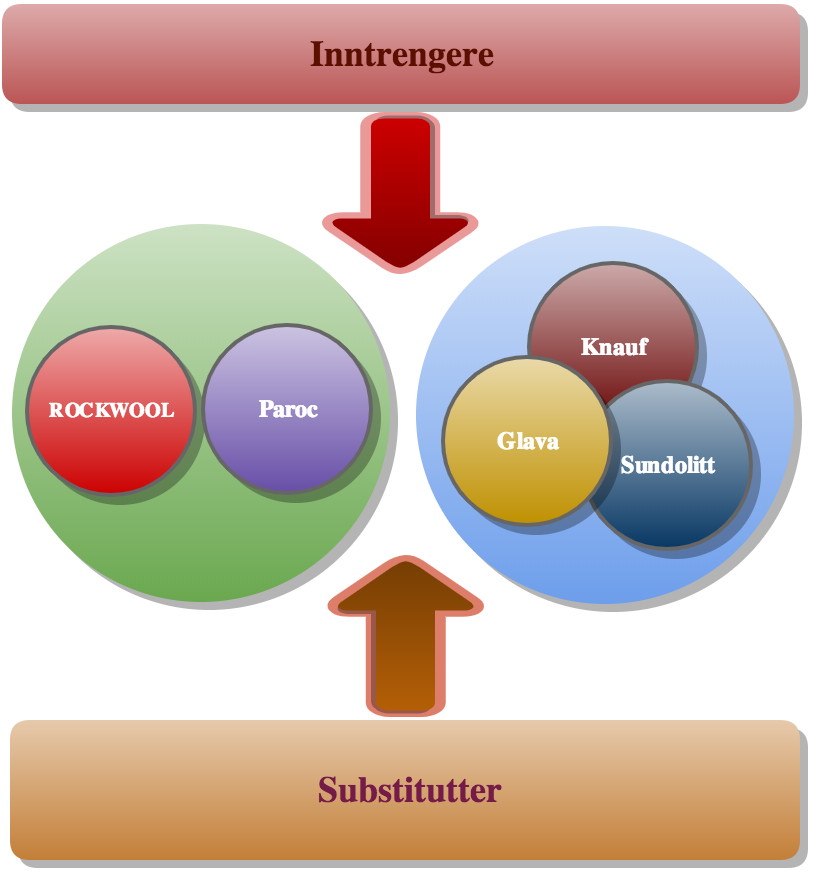
\includegraphics[width=0.48\textwidth, scale=0.2]{bilder/strategiskeGrupper.png}
  \end{center}
  \caption{Strategiske grupper}
  \label{fig:strategiskeGrupper}
\end{wrapfigure}

\indent \newline
ROCKWOOL sin konkurransearena er byggisolasjon, og er avgrenset til det norske og svenske markedet som bedriften leverer til.  Konkurrenter er henholdsvis de samme i både Norge og Sverige, hvor Glava, Knauf, Sundolitt og Paroc er de største. Glava produserer glassullisolasjon og har størst markedsandel på 40\%. Paroc er ROCKWOOL sin mest nærliggende konkurrent da de produserer steinullisolasjon. De siste årene har det kommet nye alternative isolasjonsprodukter som halmtekstil, papir og trefiber.

\indent \newline
\indent \newline
\begin{table}[ht]
\centering
\resizebox{\textwidth}{!}{%
\begin{tabular}{|l|c|c|c|c|c|}
\hline
\rowcolor[HTML]{656565} 
{\color[HTML]{FFFFFF} \textbf{Bedrift}}                          & {\color[HTML]{FFFFFF} \textbf{Råvare}} & {\color[HTML]{FFFFFF} \textbf{Isolasjon}} & {\color[HTML]{FFFFFF} \textbf{Vannavstøtende}} & {\color[HTML]{FFFFFF} \textbf{Lydisolasjon}} & {\color[HTML]{FFFFFF} \textbf{Brannsikring}} \\ \hline
\cellcolor[HTML]{FFFFFF}{\color[HTML]{000000} \textbf{ROCKWOOL}} & Stein                               & \plusmark                                         & \plusmark                                              & \plusmark                                            & \plusmark                                            \\ \hline
\cellcolor[HTML]{FFFFFF}{\color[HTML]{000000} \textbf{Paroc}}    & Stein                               & \plusmark                                         & \plusmark                                              & \plusmark                                            & \plusmark                                            \\ \hline
\cellcolor[HTML]{FFFFFF}{\color[HTML]{000000} \textbf{Glava}}    & Glass                               & \plusmark                                         & \minusmark                                              & \minusmark                                            & \plusmark                                            \\ \hline
\cellcolor[HTML]{FFFFFF}{\color[HTML]{000000} \textbf{Knauf}}    & Glass                               & \plusmark                                         & \minusmark                                              & \minusmark                                            & \plusmark                                            \\ \hline
\cellcolor[HTML]{FFFFFF}\textbf{Sundolitt}                       & Plast                               & \plusmark                                         & \plusmark                                              & \minusmark                                            & \minusmark                                            \\ \hline
\end{tabular}%
}
\caption{Produktegenskaper}
\label{produktegenskaper}
\end{table}
\indent \newline
Bedriftens strategiske gruppe identifiseres ved deres konkurranse og tilnærming til kunder \cite[s.~88]{FjeldstadogLunnan2018}. Samtlige aktører i markedet konkurrerer om de samme kundene, som i hovedsak er større entreprenører og byggevarekjeder. Derimot gjør produktegenskapene det naturlig å dele aktørene inn i to ulike strategigrupper. Paroc er den bedriften som likner mest, og plasseres derfor i samme gruppe som ROCKWOOL, mens Glava, Knauf og Sundolitt plasseres i en annen.
 
\section{Porters fem krefter}
\begin{figure}[H]
\centering
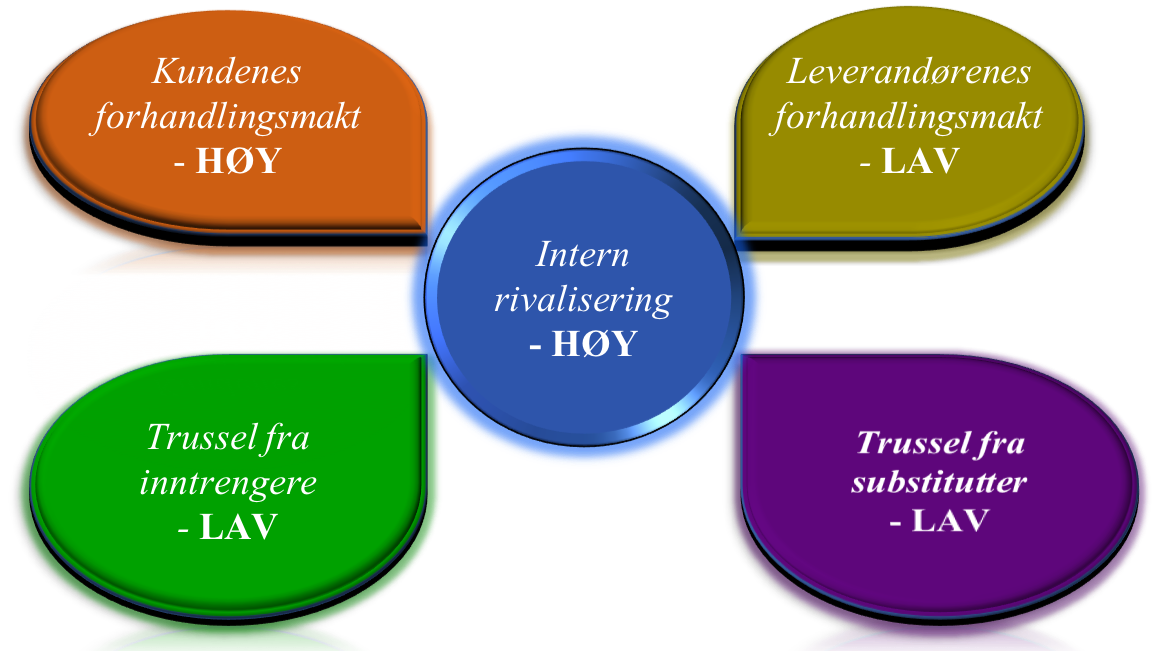
\includegraphics [scale=0.5]{bilder/portersFemKrefter.png}
\caption{Porters fem krefter - ROCKWOOL}
\label{fig:portersFemKrefter}
\end{figure}

\subsection{Trussel fra inntrengere}
Inntrengere er mulige nye konkurrenter som ønsker å etablere seg i byggisolasjonsbransjen \cite[s.~94]{FjeldstadogLunnan2018}. I en etableringsprosess for nye aktører tar man for seg mobilitetsbarrierene som påvirker inngang og utgang fra bransjen \cite[s.~90]{FjeldstadogLunnan2018}. Kapitalbehovet er stort, da det kreves store investeringer i spesialisert produksjonsutstyr. ROCKWOOL og de andre største aktørene har gjort disse investeringene over tid, noe som gir dem konkurransefortrinn overfor inntrengere. Som inntrengere må man også ta hensyn til høye faste kostnader og store avviklingsbarrierer. Stordriftsfordelene blant de største aktørene er også med på å redusere antall konkurrenter. Inngangsbarrierene er dermed høye og trussel fra inntrengere regnes som lav.

\subsection{Trussel fra substitutter}
Substituttene til ROCKWOOL er andre byggisolasjonsprodukter som dekker de samme behovene til kundene. Halm, papir og trefiber er alternative produkter, men har ikke nevneverdig markedsandel. Det vil allikevel være viktig å følge med på teknologiutviklingen som kan gjøre disse produktene mer konkurransedyktige i fremtiden.

\subsection{Kundenes forhandlingsmakt}
Bransjen består i hovedsak av to ulike kunder; byggevarekjeder og entreprenører. Byggevarekjedene fokuserer mest på pris, men langsiktige avtaler kan også forhandles frem ved bruk av bonuser og krav til å holde seminarer for byggevarekjedenes kunder. Entreprenørene fokuserer ikke bare på pris, men også hvor miljøvennlige produktene er. De står overfor strenge krav i forbindelse med totalt CO2-utslipp i byggeprosessen og vil derfor ofte favorisere produkter med lavest utslipp. Byggevarekjedene og entreprenørene er konsentrerte og har dermed høy forhandlingsmakt. Det er også relativt lite differensierte produkter som gir lave byttekostnader.

\subsection{Leverandørenes forhandlingsmakt}
Det finnes mange leverandører av råvarer i markedet, og flere av isolasjonsprodusentene handler i store kvantum. Dette gir høye byttekostnader og dermed lav forhandlingsmakt.

\subsection{Intern rivalisering}
Isolasjonsbransjen er et modent marked. De siste årene har markedsveksten ligget på ca. 2\%, og prognosene tyder på at dette vil fortsette i årene som kommer. Markedet består i hovedsak av noen få store aktører som omsetter for flere hundre millioner kroner. Produktene som tilbys er lite differensierte, bortsett fra Paroc og ROCKWOOL som tilbyr produkter med flere egenskaper. Bransjeanalysen viser til et marked med høy konkurranseintensitet hvor organisk vekst alene kan gjøre det vanskelig å utvide nåværende markedsandel. Muligheter for vekst vil derfor kunne ligge i oppkjøp eller fusjon.

\section{PESTEL-analyse}
Denne delen identifiserer faktorer i ROCKWOOL sine makroomgivelser som vil kunne påvirke bedriften i tiden fremover. Videre presenteres de viktigste funnene.

\begin{table}[ht]
\centering
\resizebox{\textwidth}{!}{%
\begin{tabular}{|l|l|l|l|l|l|}
\hline
\rowcolor[HTML]{656565} 
{\color[HTML]{FFFFFF} \textbf{Politiske}} & {\color[HTML]{FFFFFF} \textbf{Teknologiske}} & {\color[HTML]{FFFFFF} \textbf{Økonomiske}}                                     & {\color[HTML]{FFFFFF} \textbf{Miljømessige}}                      & {\color[HTML]{FFFFFF} \textbf{Sosiokulturelle}} & {\color[HTML]{FFFFFF} \textbf{Legale}} \\ \hline
- Enova                                   & - Elektrisk transport                        & \begin{tabular}[c]{@{}l@{}}- Oppgangskonjunktur\\ - Rentehevinger\end{tabular} & \begin{tabular}[c]{@{}l@{}}- Grønt skifte\\ - BREEAM\end{tabular} & - Urbanisering                                  & - CO2-avgift                           \\ \hline
\end{tabular}%
}
\caption{Makrofaktorer}
\label{Makrofaktorer}
\end{table}

\subsection{Politiske faktorer}
Enova forvalter midlene i energifondet. Formålet deres er å drive bransjene i Norge mot et lavutslippssamfunn. De tilbyr derfor økonomisk støtte til bedrifter som ønsker å velge mer energi- og klimavennlige løsninger \cite{Enova}. ROCKWOOL kan benytte seg av denne muligheten ved investering av miljøvennlige produksjonsutstyr.

\subsection{Teknologiske faktorer}
De siste årene har smelteteknologien utviklet seg fra kupolovner til el-ovner med et formål om å redusere utslipp. I følge Erik Ølstad kan teknologien redusere CO2-utslippet med ca. 80\%. Bruk av elektriske lastebiler vil de neste årene bli viktig for transportselskaper. Denne utviklingen gir ROCKWOOL muligheter til å skape en mer miljøvennlig profil som samsvarer med deres visjon.

\subsection{Økonomiske faktorer}
Norsk økonomi har vært i moderat oppgangskonjunktur det siste halvannet året og forventes å gå inn i en høykonjunktur fremover. BNP økte i 2017 med 2\% og har fortsatt med en moderat vekst så langt i 2018. Arbeidsledigheten har falt og indikasjoner tyder på at den vil fortsette å synke. Dette er faktorer som reflekterer en forbedret materiell velstand, noe som er positivt for ROCKWOOL. Derimot vil årets renteheving og de planlagte rentehevingene i 2019 kunne påvirke folk sine muligheter for låneopptak og dermed virke negativt inn på nybygg-markedet \cite{SSB}.

\subsection{Miljømessige faktorer}
Samfunnet er inne i en utvikling hvor miljøet får større fokus enn tidligere. Flere entreprenører velger derfor å BREEAM-sertifisere prosjektene sine. BREEAM er et miljøsertifiseringsverktøy for bygninger \cite{BREEAM}, som skaper utfordringer for ROCKWOOL med dagens smelteteknologi. Bedriften kan stå i fare for å miste en betydelig markedsandel hvis de ikke tar hensyn til utviklingen.

\subsection{Sosiokulturelle faktorer} 
På bakgrunn av innvandring og en trend blant unge, velger flere å flytte inn til byene. Utviklingen går derfor mot mer bebyggelse av leilighetskomplekser og færre eneboliger \cite{Urbanisering}. På sikt kan dermed kundefokus skifte mer mot entreprenørene.

\subsection{Legale faktorer}
CO2-avgiften \cite{Finansdepartementet2018} er en sentral kostnad for industriproduksjon. Med et økende miljøfokus og press i samfunnet, vil regjeringen kunne øke avgiftssatsen i nær fremtid \cite{DagbladetCO2}. En eventuell økning vil treffe ROCKWOOL hardere enn flere av konkurrentene.





